\chapter{Conclusão}
\label{chap:conclusao}

Neste trabalho fez-se o estudo de duas estratégias de controle de formação, tendo como intuito a implementação dessas estratégias não só por meio de simulações como também, com o intuito de desenvolver e aplicar essas estratégias em uma plataforma de custo relativamente baixo: o \emph{Lego Mindstorms\textregistered},  

O primeiro problema visava uma espécie de varredura em paralelo por uma frota de robôs que deveriam se alinhar e seguir se deslocando em conjunto. Já o segundo problema tinha como o objetivo controlar um time de robôs para que a mesma localizasse determinado alvo e a partir daí o circundassem, mantendo uma formação circular e equidistante entre si. Visando uma melhor cobertura da fronteira, o time deveria se reajustar caso um ou mais robôs fossem retirados da formação, de modo que os robôs remanescentes se mantenham equidistantes porém, circulando o alvo em um período menor, cobrindo melhor a fronteira.

Uma parte deste trabalho foi adaptar as estratégias e soluções encontradas para se adequar a plataforma que apresenta algumas limitações, como por exemplo a da estrutura da rede de comunicação. Uma das limitações deste trabalho, é por exemplo o fato de que a localização é feita única e exclusivamente, pelos \emph{encoders} já acoplados aos motores da plataforma. Que se mostraram, após todos os testes e experimentos realizados, suficientemente precisos para serem utilizados como ferramenta de medição e alimentação do sistema. Entretanto, o sistema fica vulnerável a deslizamentos ou a qualquer interferência externa que venha a ocorrer, podendo ocasionar uma completa desorientação do sistema sem a possibilidade de se localizar novamente. 

Embora os \emph{encoders} sejam suficientemente precisos, é necessário cautela quando se for realizar mudanças bruscas de velocidade, pois isso pode ocasionar derrapagens, fazendo com que o sistema perca sua localização. Como não há nenhum %meio externo, 
sensor externo, uma câmera ou algo para que o robô possa se localizar novamente, o erro ocorrido vai sendo acumulado até o final da execução do programa, comprometendo o cumprimento da missão do sistema multiagente.%objetivo da frota.

Outra parte importante para o estudo das estratégias de controle de formação foram as simulações realizadas que, apesar de não serem simulações realísticas que levam em consideração muitas características do sistema no mundo real, foram de extrema importância para a abstração das implementações das estratégias. Embora, considerassem o robô como um elemento pontual que ele não é, as simulações foram suficientes para verificar a viabilidade da estratégia adotada e se mostrou uma maneira fácil de verificar o comportamento do sistema para diversas estratégias, como ilustrado pela \autoref{fig:CompSimReal}, contribuindo significativamente para a conclusão deste trabalho.

\begin{figure}[!htb]
	\centering
	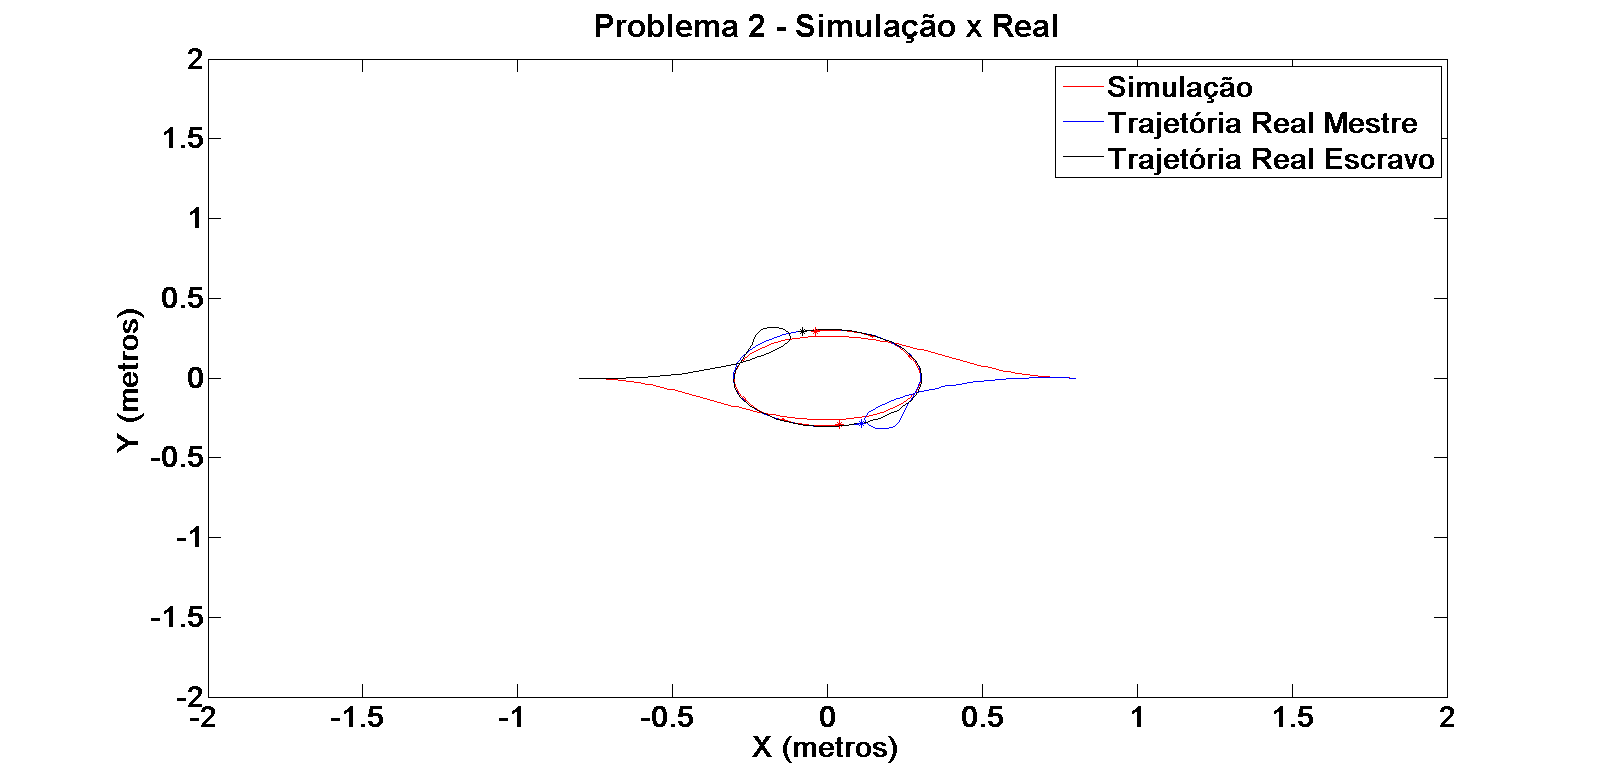
\includegraphics[width=.9\linewidth]{./Testes/Problema2/Incremental/simxReal}
	\caption{Comparação entre o problema real e a simulação}
	\label{fig:CompSimReal}
\end{figure}

No decorrer deste trabalho\footnote{Todos os arquivos para simulações e a implementação deste trabalho se encontram em um repositório do \emph{GitHub}. Para acessar o código-fonte das simulações, das malhas de controle e dos problemas, assim como acessar a alguns dados dos testes realizados neste trabalho, acesse o link: https://github.com/MarianaAthayde/tcc/tree/master.} foram testados alguns controladores distintos e ajustado empiricamente diversos ganhos para um controlador PID que atendesse aos requisitos do sistema e o que pode-se constatar é que embora alguns controladores tenha demostrado erros menores ou tempo de ajuste inferiores, como pode ser observado comparando-se as tabelas \ref{t:cinc}, \ref{t:cpid} e os resultados obtidos na \autoref{m1ContPol}, o que determinou o melhor controlador para o problema foi um custo benefício entre erro, tempo de ajuste e também, suavidade de controle. 

No geral, o controlador da malha interna que melhor atendeu e cumpriu com o objetivo deste trabalho, foi o controlador aqui denominado como polinomial. % Este controlador consiste em uma função polinomial que converte a velocidade angular desejada em uma variável de potência dos motores, que foi mapeada pelo fabricante em um intervalo de -100 a 100, para que então um controlador PID já ajustado pelo fabricante  
Este controlador é na verdade, um controlador PID já implementado e ajustado pelo fabricante e o ajuste polinomial foi utilizado somente para se obter uma função que traduza o valor de referência (\emph{set point}) aceito pelo controlador do fabricante em velocidade angular das rodas. Já na malha intermediária (malha 2), a malha retratada na seção \ref{sec:malha2}, um controlador proporcional se mostrou suficiente para atingir os objetivos deste trabalho, ao passo que ao inserir um ganho integrador no sistema, o mesmo se mostrou instável.

Foram realizados neste trabalho apenas testes com implementações em uma frota de dois robôs, no entanto, seria interessante como trabalho futuro, aplicar este estudo a uma frota de quatro robôs, como o suportado pela rede de comunicação implementada pela plataforma. 

\section{Trabalhos Futuros}
 \label{sec:trabFuturos}
 Como trabalhos futuros sugere-se a implementação de um tratamento de colisão que, embora não implementado neste trabalho, é parte essencial de um controle de formação, visto que para cumprir com um objetivo real as tropas devem ser capazes de trabalhar em conjunto sem que um robô atrapalhe a ação de outro e prejudique o desempenho da frota. A inserção de sensores e de uma malha de controle para que o robô consiga interagir com o ambiente, de modo a tornar o controle de formação mais eficiente e mais próximo aos sistemas que resolvem problemas no mundo real, também é uma perspectiva de continuidade interessante.
 
 Outro trabalho interessante seria fazer robôs que se comportem como indivíduos inteligentes e autônomos, capazes de realizar missões individualmente mas também, capazes de se organizarem em uma sociedade que possui objetivos em comum e sejam capazes de decidir pela "melhor" estratégia de formação para cada problema.
 
